\documentclass[a4paper,12pt]{article}
\usepackage[a4paper, margin=2.54cm]{geometry}
\usepackage[german]{babel}
\usepackage[UTF8]{inputenc}
\usepackage{setspace}
\usepackage{graphicx}
\usepackage{caption}
\usepackage{subcaption}
\onehalfspacing
\begin{document}

	\section{Einführung}
	\subsection{Motivation}
	In der heutigen Zeit wird der Verwendung von Mikrocontrollern eine immer höre Bedeutung zugemessen. Diese entsteht durch die einfache Programmierung auf Systemebene in Assebly sowie die konstengünstige und platzspaarende Produktion.\\
	Die Verwendung des 8051  bietet hierbei eine bekannte Plattform, welche sich für die Umsetzung einer Vielzahl an kreativen Projekten eignet.\\
	Die Idee dieses Projektes besteht darin, die Hardware mit verschiedener Peripherie zur Eingabe von Morse-Code zu nutzen.\\
	Der Morse Code ist ein Code, welcher zur Übermittlung von Daten in Textform genutzt werden kann und die Verständigung über primitive Technik erlaubt. 
	\subsection{Aufgabenstellung}
	Die Aufgabenstellung war es ein Programm für den 8051 Microcontroller zu schreiben, das folgende Anforderung erfüllt:
	\begin{itemize}
		\item Compilierfähigkeit des Programmes
		\item Verwendung eines Timers
		\item Verwendung eines Interrupt
	\end{itemize}
	Zur Vereinfachung wurde anstatt eines 8051 ein Simulationsprogramm verwendet, welche sowohl den 8051, als auch die Ein und Ausgabehardware simuliert.\\
	Der fertige Code ist offen auf Github zu finden.
	
	\newpage
	
	\section{Grundlagen}
	\subsection{Assembler}
	Als Assembler oder Assebly bezeichnet man eine Programmiersprache, mit welcher sich eine bestimmte Hardware oder Prozessorachitektur gezielt programmieren lässt. Asseblercode wird also gezielt für eine Architektur entwickelt und lässt sich nur auf dieser ausführen.\\
	Der Quellcode bildet hierbei eine Folge von Maschinenbefehlen. Maschinenbefehle bestehen dabei aus einem Operationscode und meist einer weiteren Folge von Angaben wie Adressen oder Literalen.\\
	\ref{ls:mov} zeigt hierbei einen einfachen MOV - Befehl in  der Maschinensprache von x86 Prozessoren. MOV bedeutet hierbei so viel wie mov-byte von/was, nach. Verschiedene Assembler Dialekte unterscheiden sich in der Bedeutung gleicher Befehle.\\
	
	\subsection{8051 Mikrocontroller}
	Der Intel 8051 ist ein von in den Jahren von 1980 bis 1990 unter anderen von Intel und Simens hergestellter Mikrokontroller. Verwendung fand er in unbterschiedlichen Gebieten der Automobilindustrie, Robotik sowie der Telekommunikation.\\
	In der ursprünglichen und hier betrachteten Form handelt es sich bei dem 8051 um einen Rechner nach der Havard-Architektur \cite, welche den Programm vom Datenspeicher trennt.\\
	Der Prozessortakt ist mit 12MHz und der Befehlsatz mit 8 Bit = 1 Byte angegeben. Außerdem verfügt er über einen 4 KB Programmspeicher, 128 Byte Datenspeicher und zwei 16-Bit Timer. Andere Prozessoren der Baureihe können auch leistungsfähiger sein.\\
	Im Folgenden geben wir ein Übersicht der Virtuellen Hardware, welche für das Projekt verwendet wurde.
	
	\subsubsection{Simple Keypad}
		\begin{figure}[bt]
			\centering
			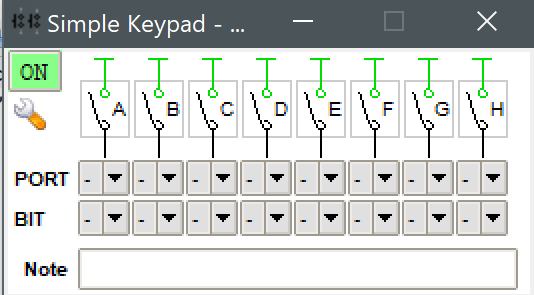
\includegraphics[width=0.7\linewidth]{Bilder/keypad}
			\caption[IDE Screenshot]{IDE Screenshot}
			\label{fig:ide8051keybad}
		\end{figure}
	Mit dem Simple Keypad \ref{ide8051keybad} lassen sich über dedizierte Ports jeweils Schalter simulieren, welche entweder an oder aus sind. 
	
	\subsubsection{LC Display}
	\begin{figure}[bt]
		\centering
		\includegraphics[width=0.7\linewidth]{Bilder/lcd}
		\caption[IDE Screenshot]{IDE Screenshot}
		\label{fig:ide8051lcd}
	\end{figure}
	
	
	\subsection{Entwicklungsumgebung MCU 8051}
	Zur Implementierung des Programms wurde nicht direkt an der Hardware des 8051 gearbeitet, sondern mit einer virtuellen Entwicklungsumgebung des 8051, der MCU 8051 von Mavriria Microsystems.\\
	Vorteile des Einsatz der Virtuellen Hardware war der direkte Einblick in die verschiedenen Register und Ports des 8051 sowie der virtuellen Hardware. 
	\begin{figure}[bt]
		\centering
		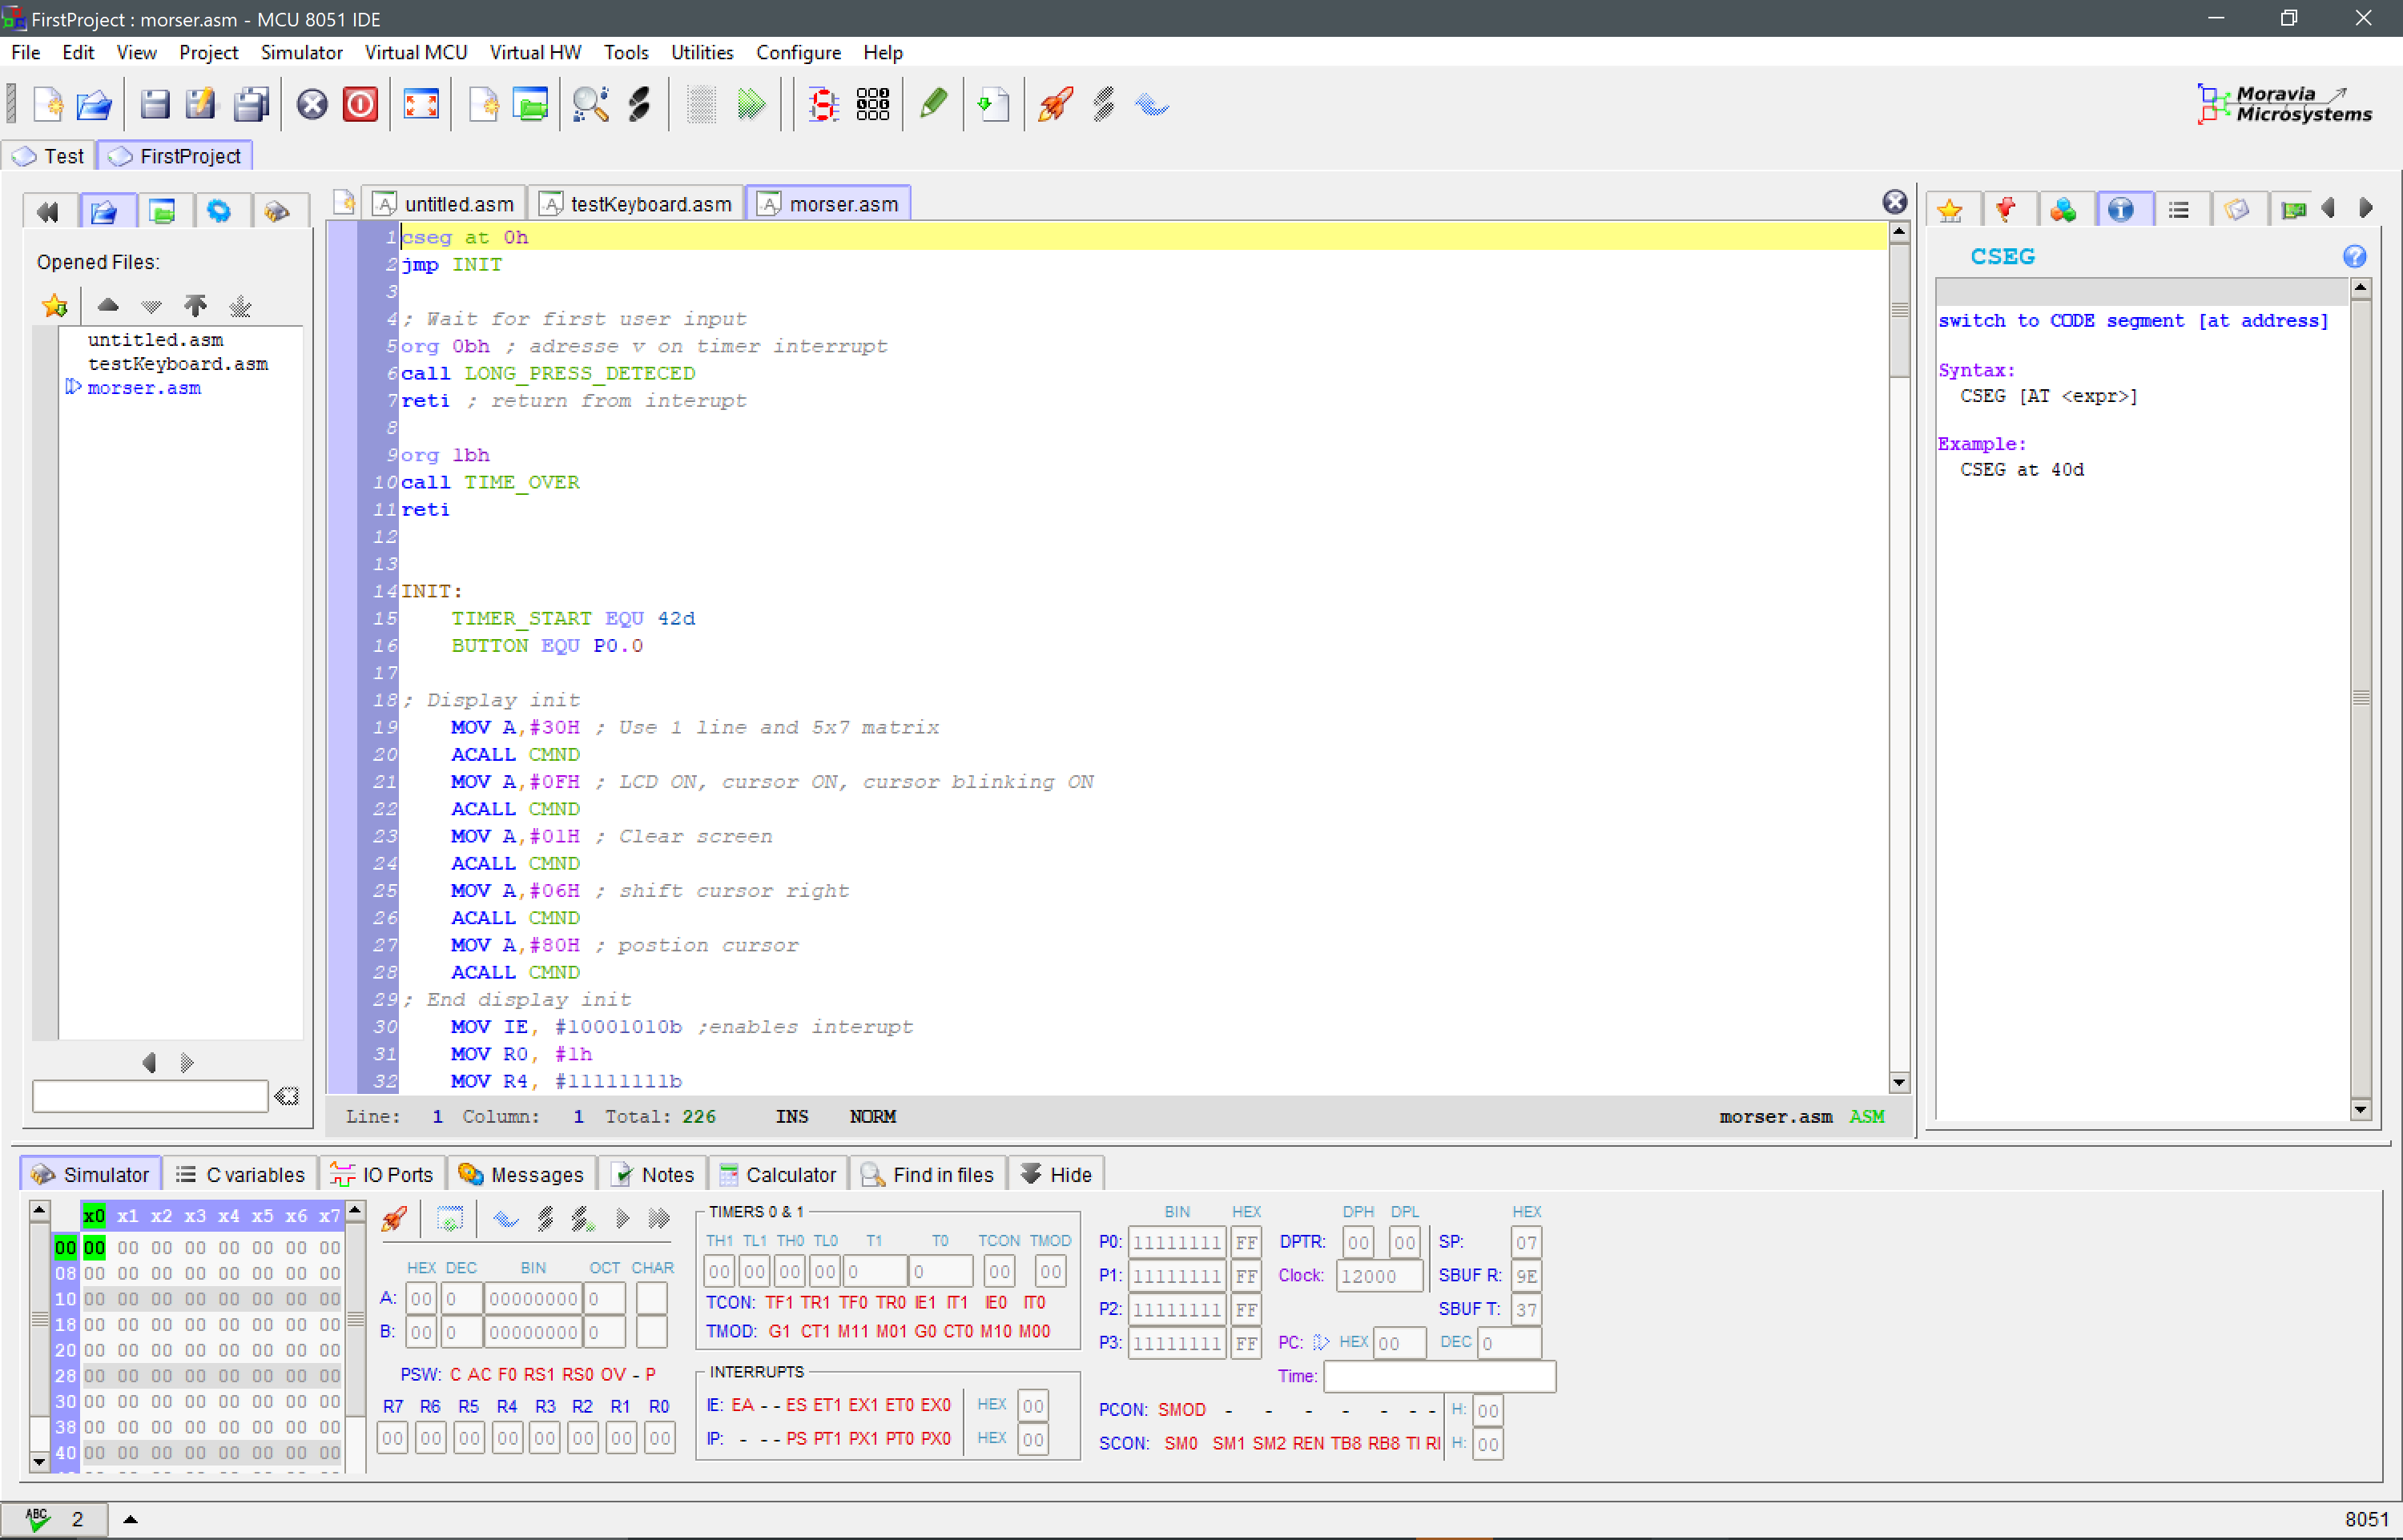
\includegraphics[width=0.7\linewidth]{Bilder/IDE8051}
		\caption[IDE Screenshot]{IDE Screenshot}
		\label{fig:ide8051}
	\end{figure}

	\subsection{Morsecode}
	Der Morsecode [\ref{fig:morse-code}] ist ein Zeichensatz, welcher zu Übertragung von Daten verwendet wird. Das Morsealphabet besteht dabei aus drei dijunkten Zeichen: kurzes Signal, langes Signal, Pause. Das bekannteste Morsesignal ist \textit{kurz - kurz - kurz - lang - lang - lang - kurz - kurz - kurz}, welches für den Seenotruf SOS steht. Das Signal kann dabei als Tonsignal, als Funksignal oder als elektischer Impuls von einem Morsetaster über eine Telefonleitung, mechanisch oder optisch übertragen werden.\\
	Der Morsecode ist eine Entropiekodierung, da öfters vorkommende Zeichen mit weniger Signalen codiert sind (ausgehend von der Häufigkeit in der englischen Sprache).\\

	\begin{figure}[bh]
		\begin{subfigure}{0.5\linewidth}
			\centering
			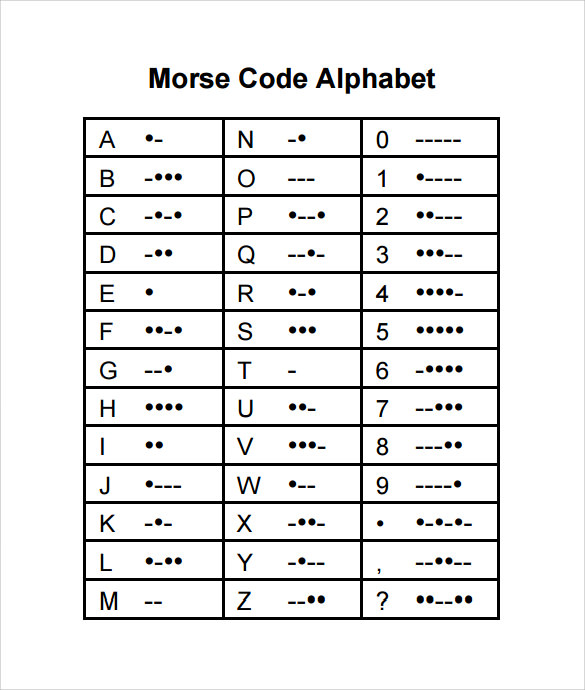
\includegraphics[width=0.95\linewidth]{Bilder/Morse-Code-Alphabet-Chart.jpg}
			\caption{Internationaler Morse Code}
			\label{fig:morse-code}
		\end{subfigure}
		\begin{subfigure}{0.5\linewidth}
			\centering
			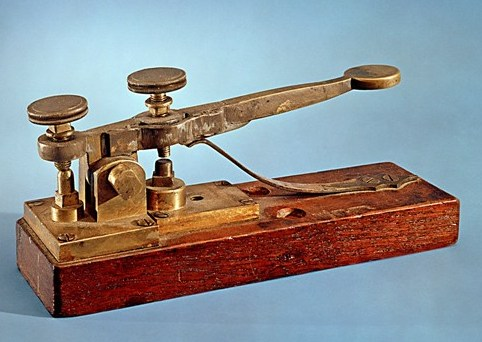
\includegraphics[width=0.95\linewidth]{Bilder/morse-telegraph-machine.jpg}
			\caption{Morsecode-Telegraph}
			\label{fig:morser}
		\end{subfigure}
	\end{figure}

	Unzulänglichkeiten des Morse-Codes bestehen darin, dass die Fano-Bedingung für den Morse-Code nur dann enfüllt ist, wenn man das dritte Symbol, die Pause als festes Symbol definiert. Daraus ergibt sich, dass keine Wort den identischen Anfang eines anderen Wortes ist. Nach jedem erkannten Wort kann also direkt mit dem nächsten Wort weitergemacht werden.
	
	
	
	\newpage 
	\section{Konzept}
	\subsection{title}
\end{document}


